\documentclass[border=10pt]{standalone}
\usepackage{graphicx}
\usepackage{epstopdf}
\usepackage{mathptmx}
\usepackage{amsmath}

\begin{document}
	\begin{minipage}{66cm}
		\centering
		\begin{minipage}[t]{0.99\linewidth}
			\centering
			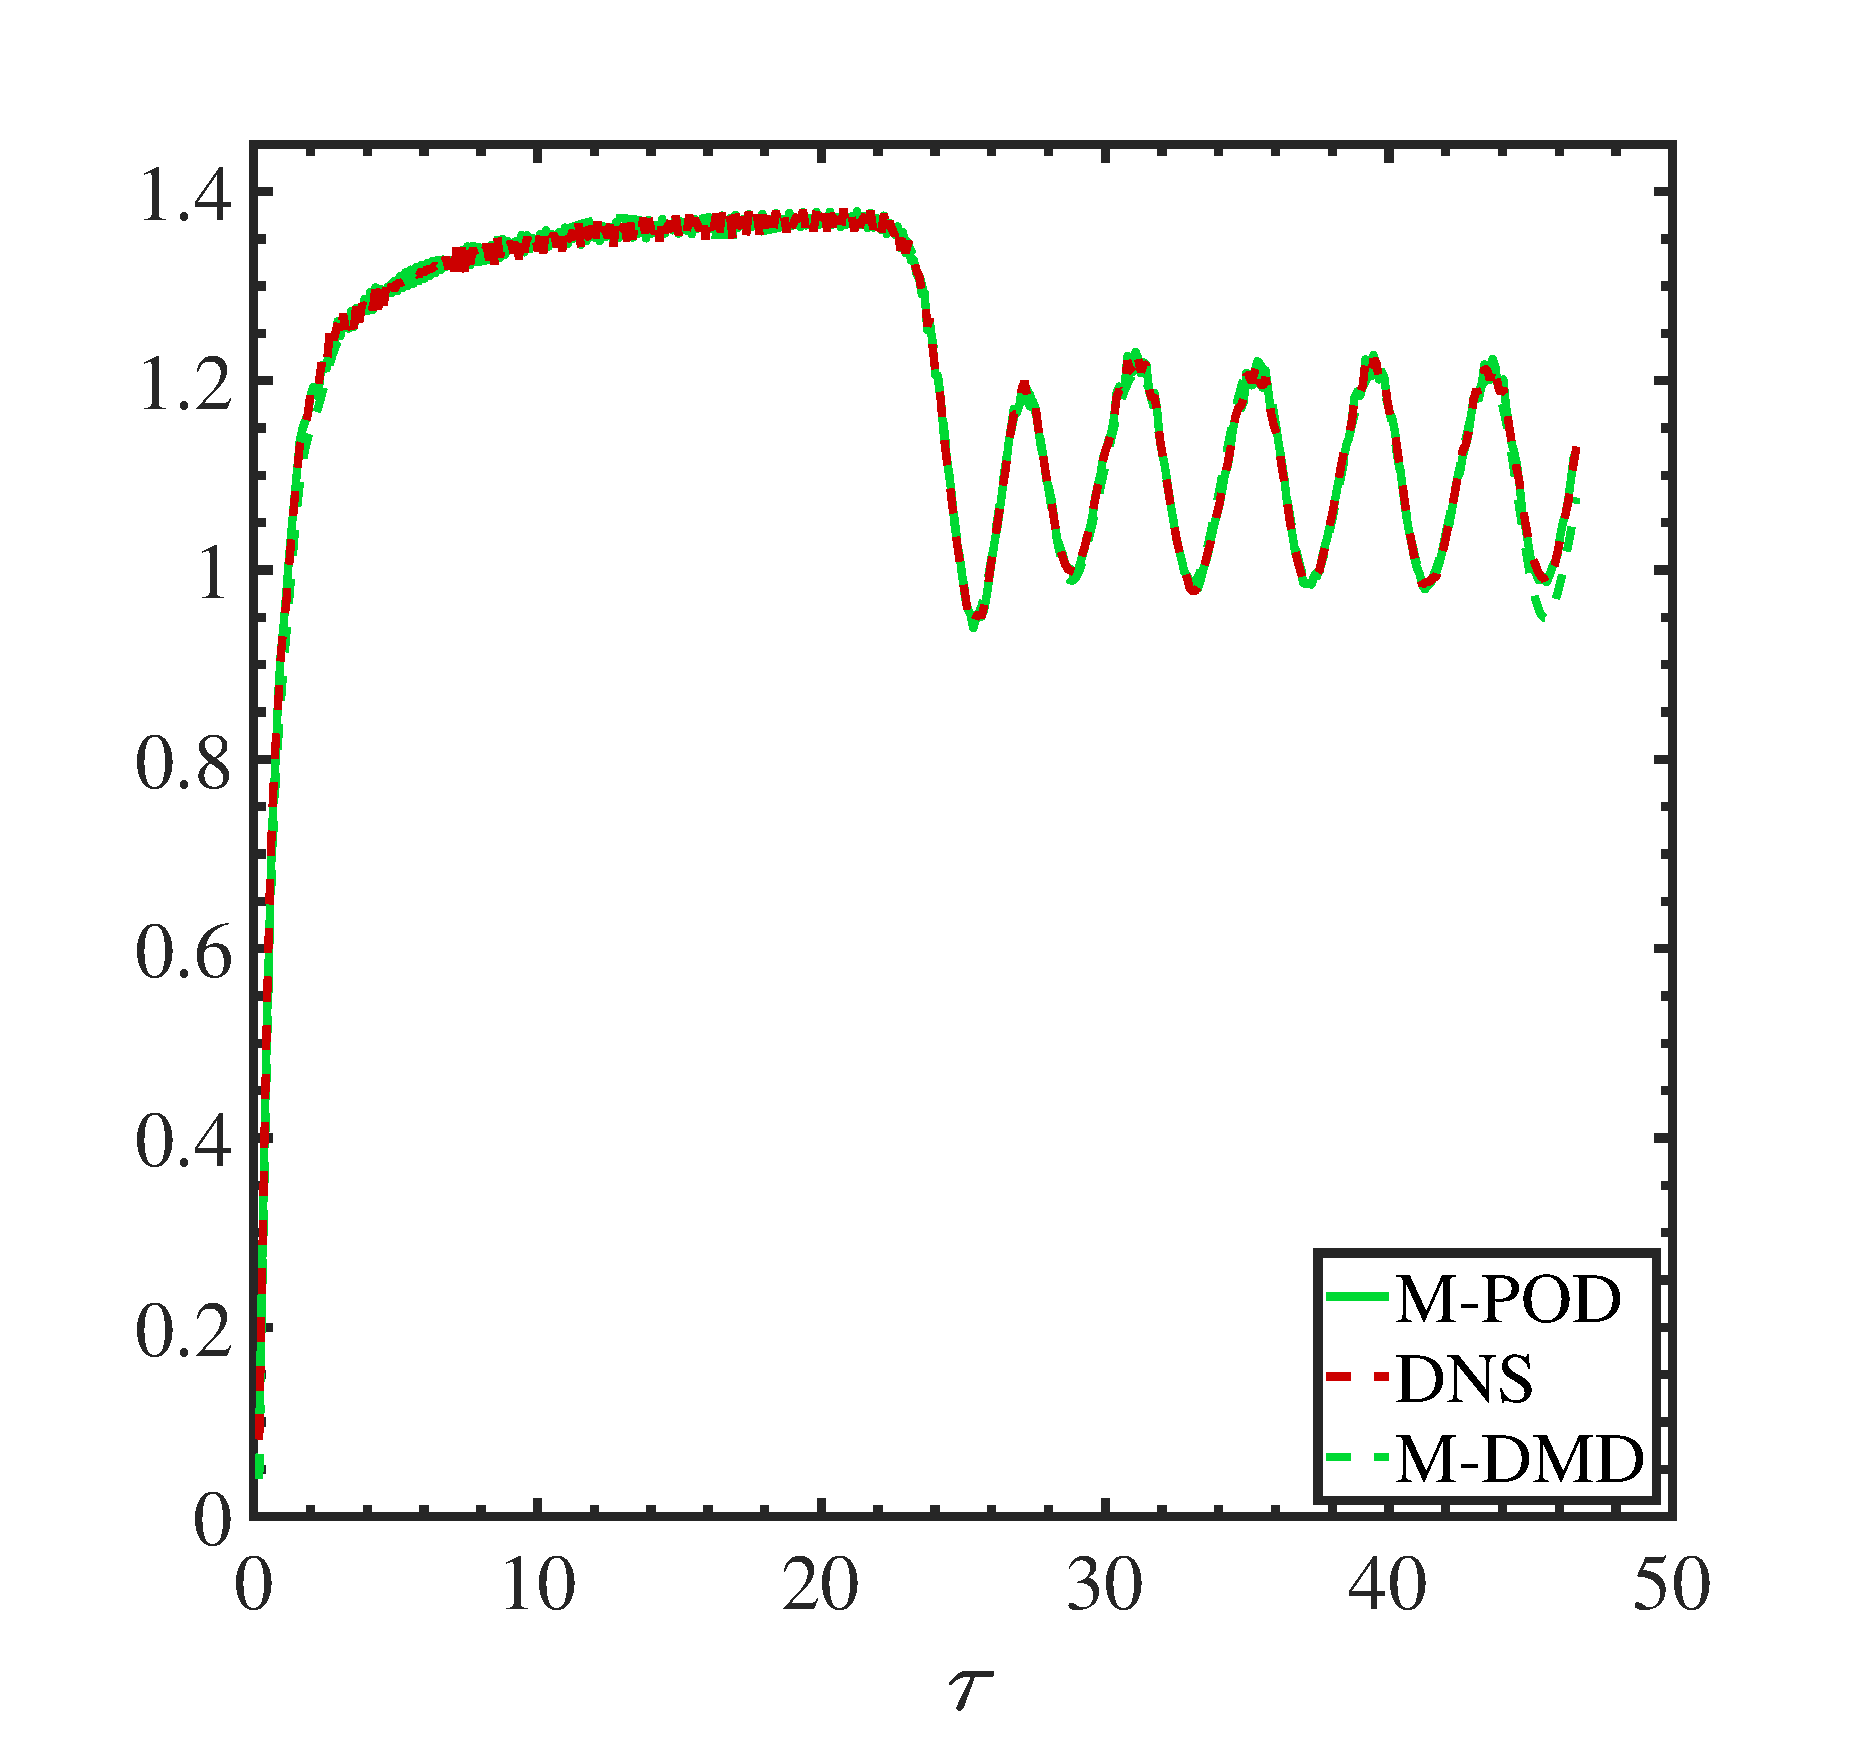
\includegraphics[scale=1,trim={0.5cm 1.9cm 1cm 0cm},clip]{Figure8a1.eps}
			\put(-940,370){\fontsize{40}{12}\selectfont\textbf{(a)}}
			\put(-880,330){\rotatebox{90}{\fontsize{45}{12}\selectfont\textbf{$U_{c}$}}}
			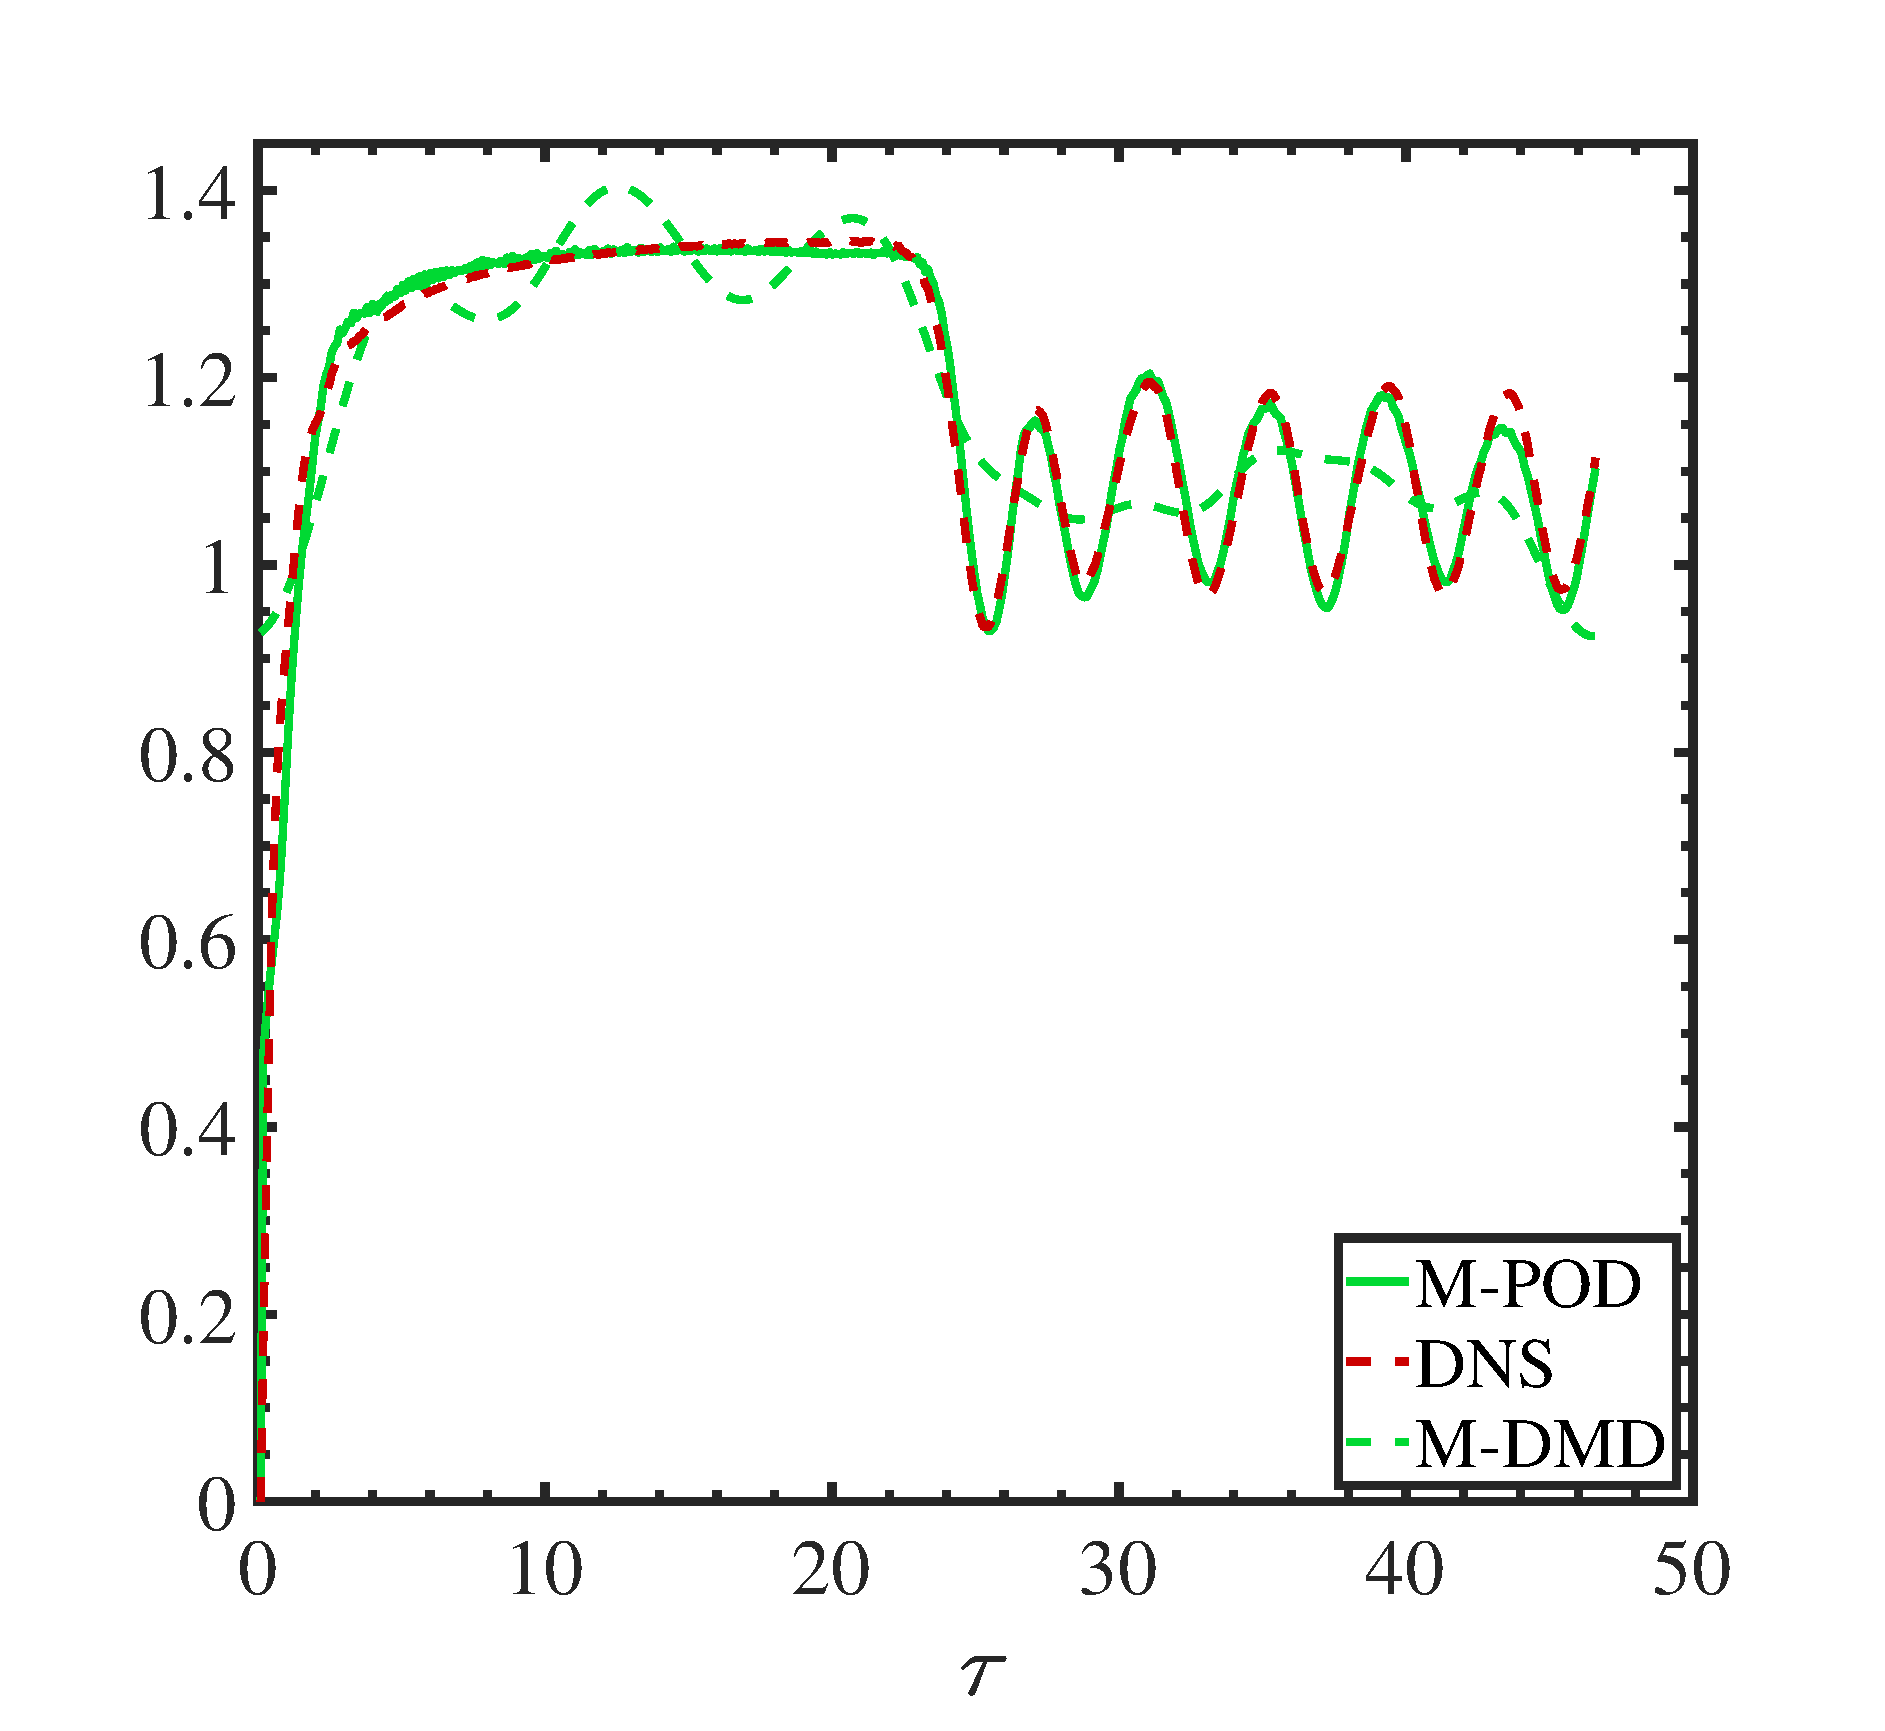
\includegraphics[scale=1,trim={0cm 1.9cm 2cm 0cm},clip]{Figure8b1.eps}
			\put(-850,350){\rotatebox{90}{\fontsize{45}{12}\selectfont\textbf{$U_{av}$}}}
		\end{minipage}
		\vspace{0.2cm}
		\begin{minipage}[t]{1\linewidth}
			\centering
			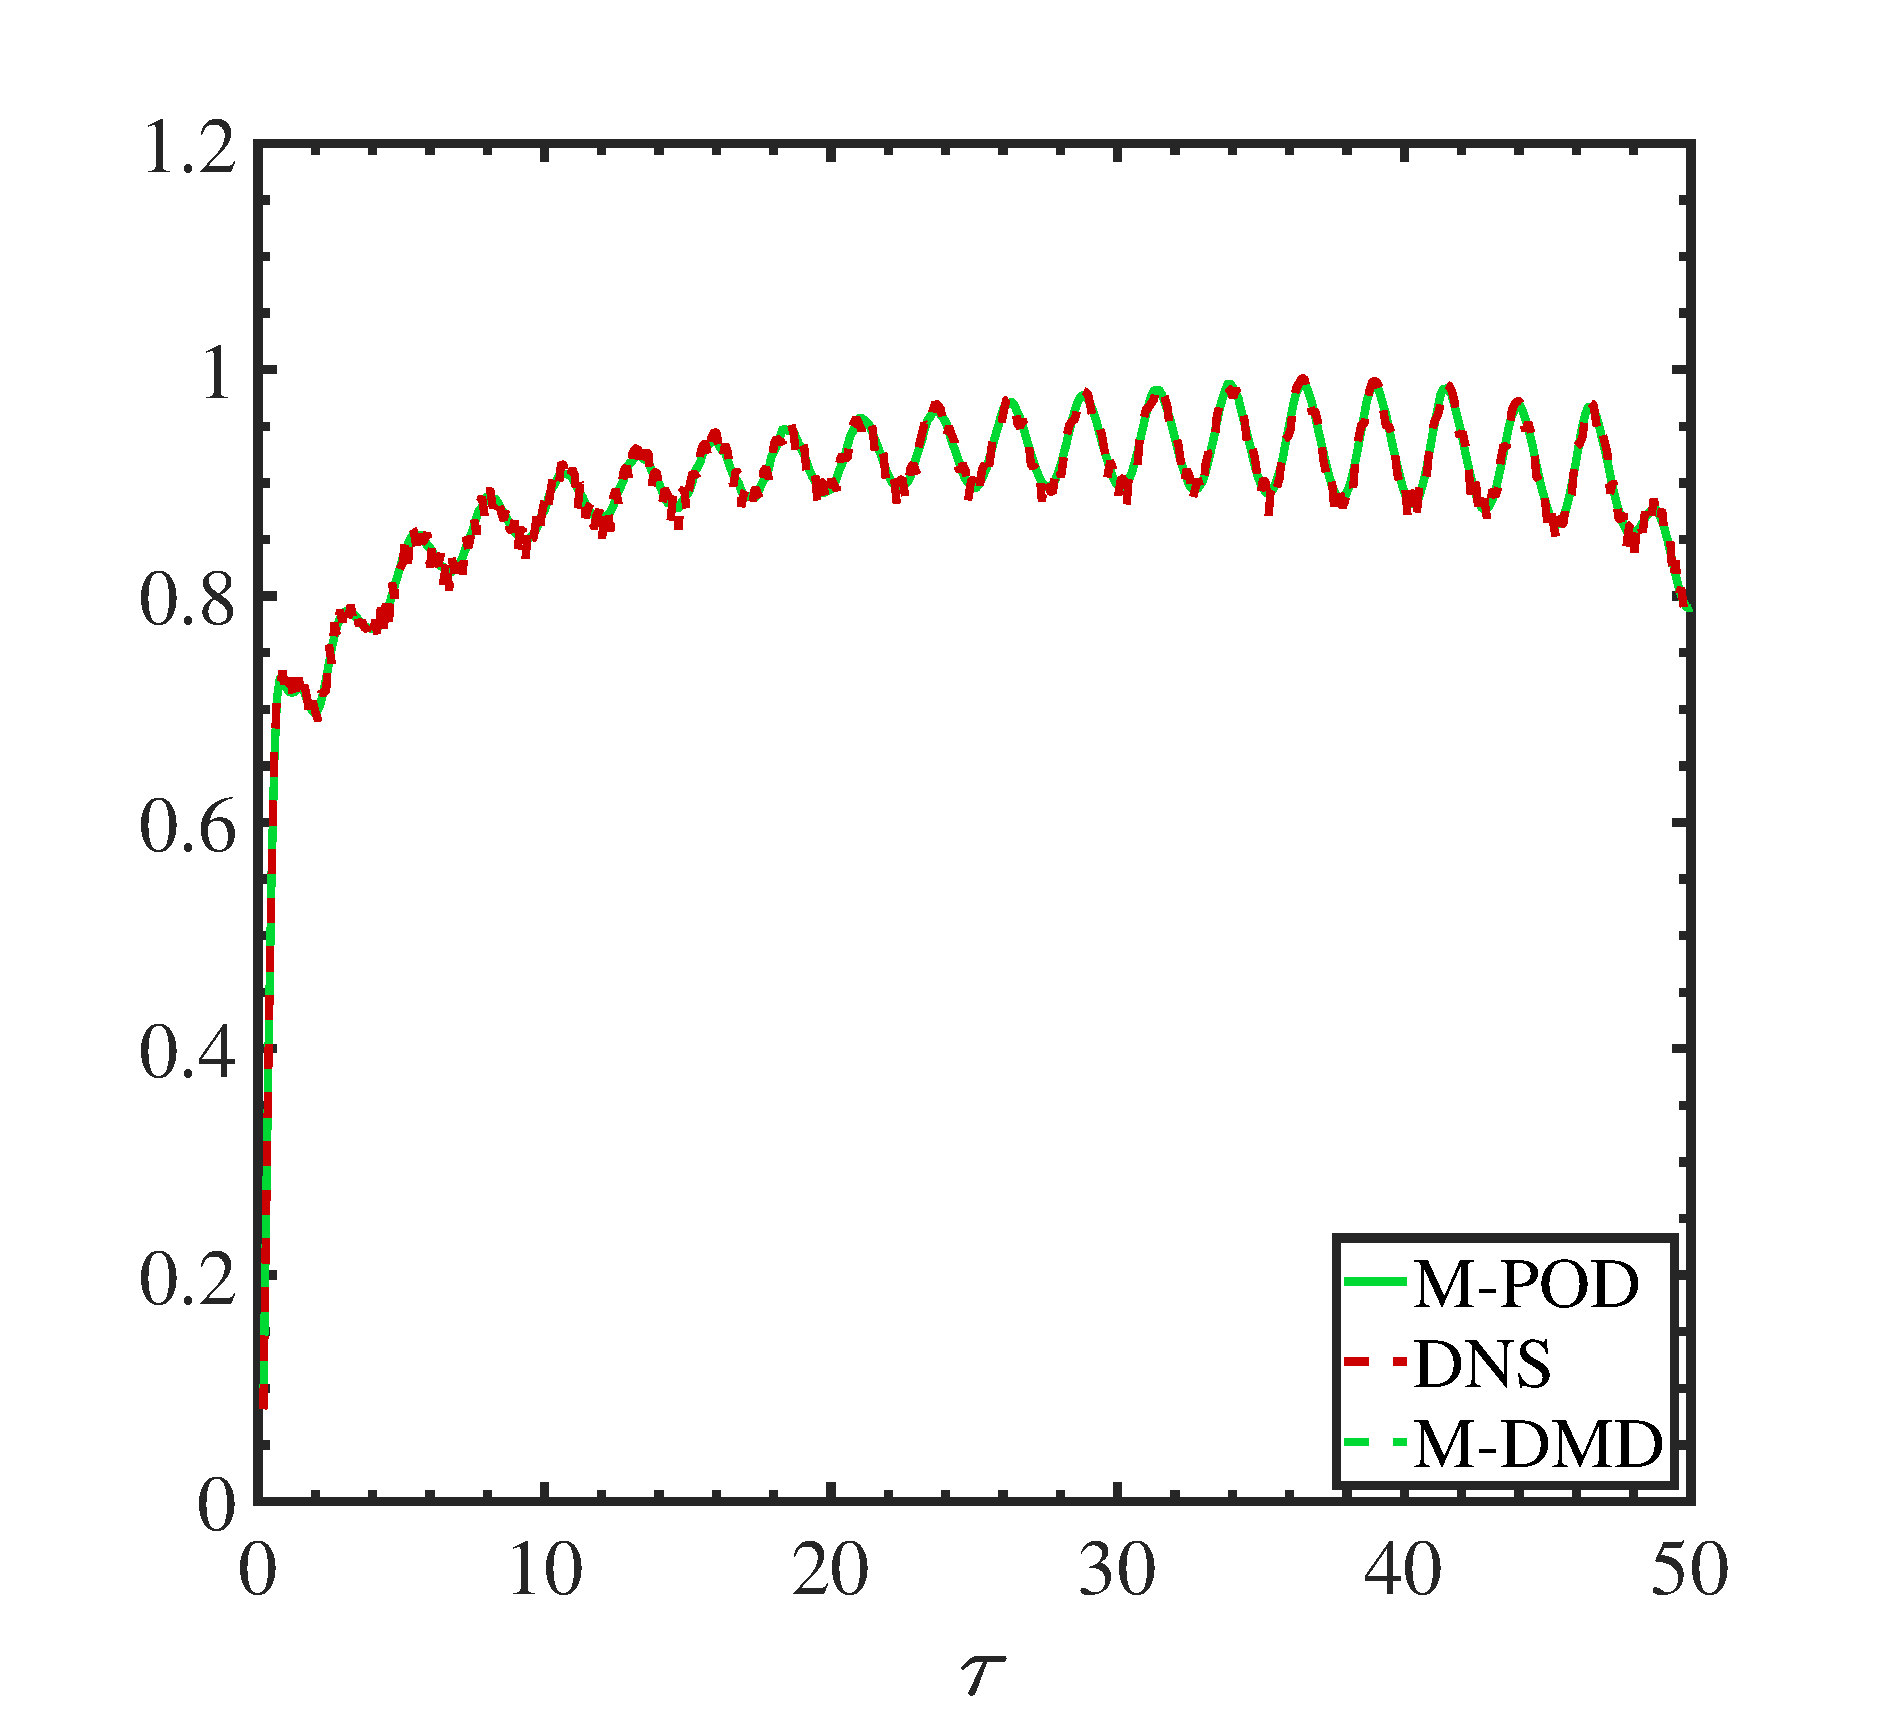
\includegraphics[scale=1,trim={0.5cm 0cm 1cm 0cm},clip]{Figure8a2.eps}
			\put(-940,430){\fontsize{40}{12}\selectfont\textbf{(b)}}
			\put(-880,400){\rotatebox{90}{\fontsize{45}{12}\selectfont\textbf{$U_{c}$}}}
			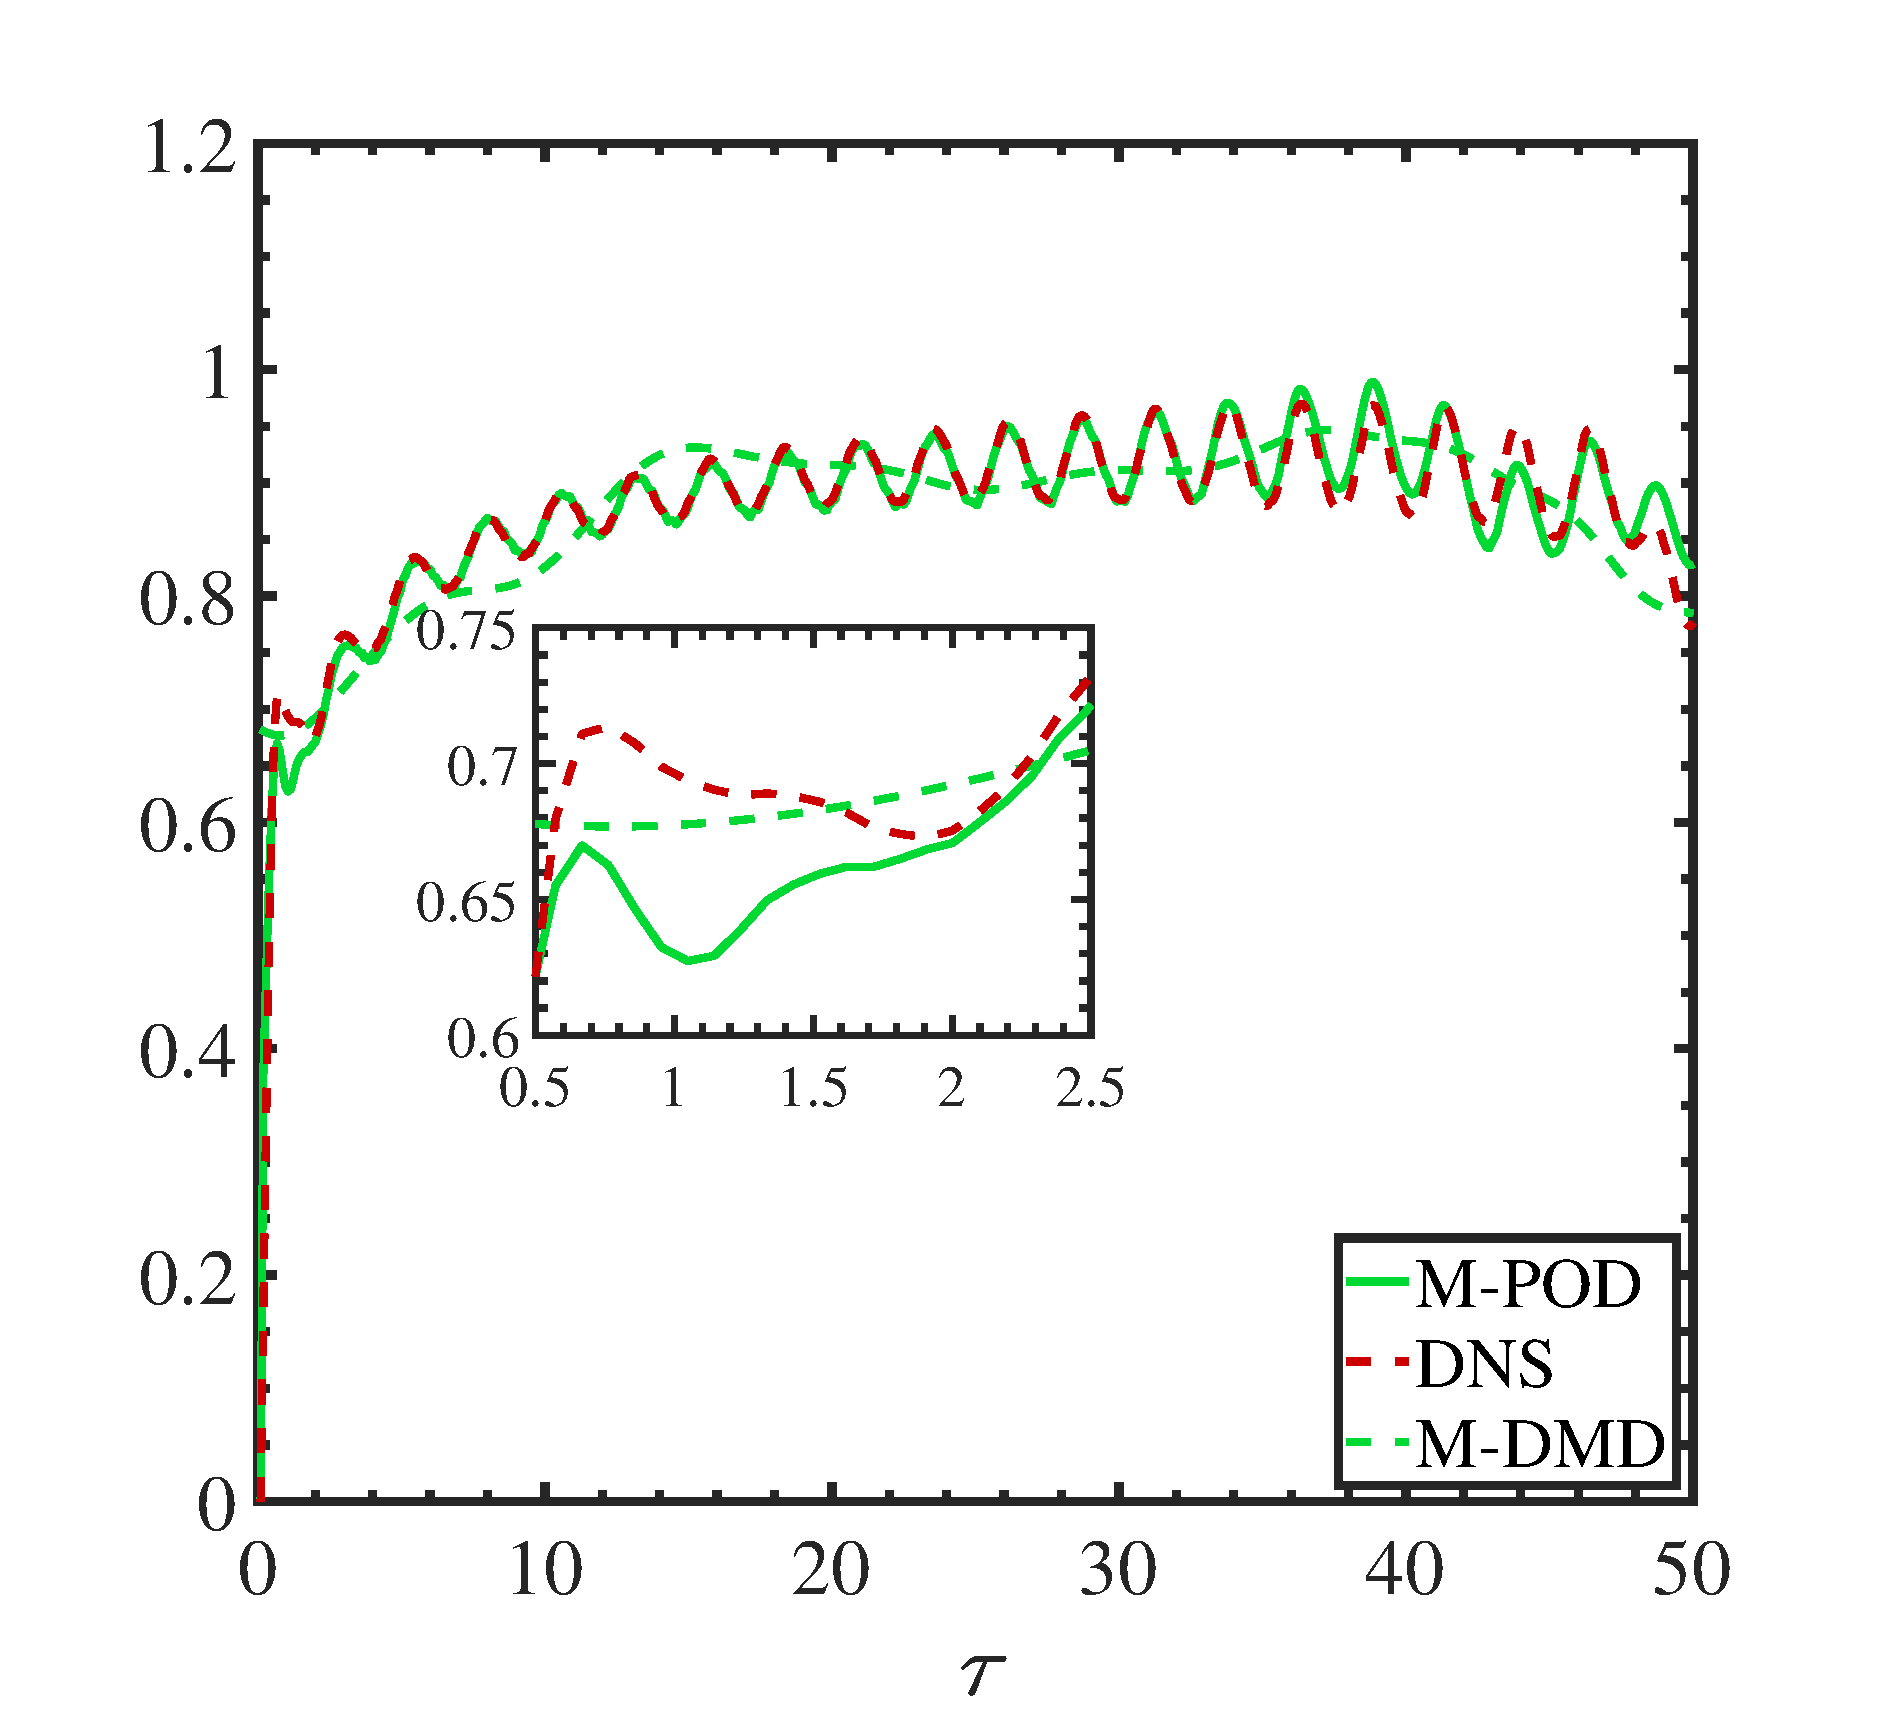
\includegraphics[scale=1,trim={0cm 0cm 2cm 0cm},clip]{Figure8b2.eps}
			\put(-850,400){\rotatebox{90}{\fontsize{45}{12}\selectfont\textbf{$U_{av}$}}}
		\end{minipage}
	\end{minipage}
\end{document}